\documentclass[12pt]{article}
\usepackage[margin=2.5cm]{geometry}
\usepackage{tikz}
\usepackage{amsmath}
\usepackage{mathtools}
\usepackage{graphicx}
\setlength{\parindent}{0pt}
\setlength{\parskip}{0.75em}



\title{Chapter 2: Kinematics}
\author{İskender Yalçınkaya, PhD}
\date{\today}

\begin{document}
\maketitle
\section{Notion of a Particle}
A \emph{particle} is a body whose size and shape are not important for the problem at hand. In other words, a particle is a body that can be treated as a point mass. The motion of a particle is described by its position, velocity, and acceleration as functions of time. For example, planets can be treated as particles when studying their motion around the sun, even though they have size and shape. But when studying the tidal waves on earth and the tornadoes in the atmosphere, the size and shape of the earth is important, and they cannot be treated as particles.

Mathematically, a particle is a point in the space with an associated mass. Therefore, if one has to define a density function for a point particle which is located at $\mathbf{r}_0$, it would look like:
\[
\rho(\mathbf{r}) =
\begin{cases}
\infty, & \mathbf{r} = \mathbf{r}_0,\\[4pt]
0, & \mathbf{r} \neq \mathbf{r}_0.
\end{cases}
\]

\begin{figure}[h!]
    \centering
    \includegraphics[scale=0.5]{figures/point-particle.png}
\end{figure}


How can we mathematically write down the total mass of the particle in terms of its density function? We can consider the integral of the density function over all space, right? If $\rho$ is infinite at $\mathbf{r}_0$, wouldn't the integral be infinite as well? According to what we have learned in calculus, the integral of a function that is infinite must br infinite as well.
\begin{equation}
\int_{\text{all space}} \rho(\mathbf{r}) dV = \infty
\end{equation}
We attribute a geometrical ``dot'' a physical property called mass and we still want the mathematics work: We do not want the above integral to be infinite. Therefore, we say let it not be infinite, let it be a finite number $m$. In other words, we define the integral as follows:
\begin{equation}
\int_{\text{all space}} \rho(\mathbf{r}) dV \equiv m
\end{equation}
You will see more about this in Electricity and Magnetism course when we define Dirac delta function. 

\section{The Position Vector}
The position of a particle is described by a vector called the \emph{position vector}:
\begin{equation}
\mathbf{r}(t) = x(t) \mathbf{i} + y(t) \mathbf{j} + z(t) \mathbf{k}
\end{equation}
where $x(t)$, $y(t)$, and $z(t)$ are the coordinates of the particle as functions of time in a Cartesian coordinate system, and $\mathbf{i}$, $\mathbf{j}$, and $\mathbf{k}$ are the unit vectors in the $x$, $y$, and $z$ directions, respectively. The position vector points from the origin of the coordinate system to the position of the particle at time $t$. The magnitude of the position vector represents the distance of the particle from the origin, and its direction represents the direction of the particle from the origin. The position vector is a function of time, and it can be used to describe the motion of the particle in space. The position vector can also be expressed in terms of spherical or cylindrical coordinates, depending on the problem at hand. 



\begin{figure}[ht]
\centering
\begin{minipage}{0.42\textwidth}
    \centering
    \includegraphics[width=\linewidth]{figures/position-vector.png}
\end{minipage}\hfill
\begin{minipage}{0.54\textwidth}
\centering
\begin{tikzpicture}[>=stealth, scale=1.2]

    % Axes
    \draw[->] (-0.3,0) -- (5,0) node[right] {$x$};
    \draw[->] (0,-0.3) -- (0,4) node[above] {$y$};

    % Particle
    \fill (3.5,2.5) circle (2pt) node[above right] {Particle};

    % Position vector
    \draw[->, thick] (0,0) -- (3.5,2.5)
        node[midway, above left] {$\mathbf{r}(t)$};

    % Coordinates
    \draw[dashed] (3.5,0) -- (3.5,2.5);
    \draw[dashed] (0,2.5) -- (3.5,2.5);

    % Coordinate labels
    \node[below] at (3.5,0) {$x(t)$};
    \node[left] at (0,2.5) {$y(t)$};

    % Origin
    \node[below left] at (0,0) {$O$};

\end{tikzpicture}
    \end{minipage}
\caption{The position vector $\mathbf{r}(t)$ of a particle in a two-dimensional Cartesian coordinate system.}
\label{fig:position_vector}
\end{figure}




\section{The Displacement Vector}
What happens if a particle moves from one position $r_1(t_1)$ to another position $r_2(t_2)$? The displacement of a particle is described by a vector called the \emph{displacement vector}. It is defined as the change in position of the particle, and is given by the difference between the final position vector and the initial position vector:
\begin{equation}
\Delta \mathbf{r} = \mathbf{r}_2 (t_2) - \mathbf{r}_1 (t_1)
\end{equation}

The displacement vector points from the initial position to the final position, and its magnitude represents the distance traveled by the particle in a straight line. The displacement vector is independent of the path taken by the particle, and only depends on the initial and final positions.

\begin{figure}[h]
\centering
\begin{minipage}{0.6\textwidth}
\centering
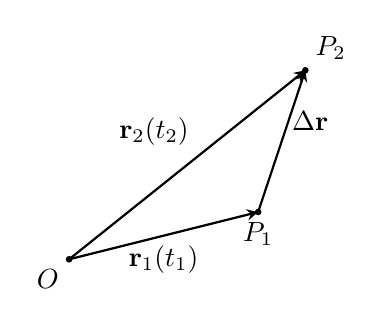
\begin{tikzpicture}[>=stealth, thick, scale=0.6]

    % Points
    \coordinate (O)  at (0,0);
    \coordinate (P1) at (4,1);
    \coordinate (P2) at (5,4);

    % Position vector r_1
    \draw[->] (O) -- (P1)
        node[midway, below] {$\mathbf{r}_1(t_1)$};

    % Position vector r_2
    \draw[->] (O) -- (P2)
        node[pos=0.55, above left] {$\mathbf{r}_2(t_2)$};

    % Displacement vector
    \draw[->] (P1) -- (P2)
        node[midway, above right] {$\Delta\mathbf{r}$};

    % Points
    \fill (O) circle (2pt) node[below left] {$O$};
    \fill (P1) circle (2pt) node[below] {$P_1$};
    \fill (P2) circle (2pt) node[above right] {$P_2$};

\end{tikzpicture}
\end{minipage}
\caption{Position vectors and displacement vector.}
\label{fig:position_displacement}
\end{figure}

If we simple subtract $\mathbf{r}_1$ from $\mathbf{r}_2$ by using the head to tail method, the resulting vector would be in some direction starting from the origin. But the displacement vector is defined as the vector that starts from the initial position and ends at the final position. Therefore, we need to translate the vector $\mathbf{r}_1$ to the point $\mathbf{r}_2$ in order to find the displacement vector $\Delta \mathbf{r}$. This is shown in Figure \ref{fig:position_displacement}.


\section{The Velocity Vector}

The \emph{velocity} is defined as the change in position with respect to time. If the displacement of the particle is described by $\Delta \mathbf{r}$, can we define the velocity as follows?

\[
\mathbf{v}\overset{?}{=}\frac{\Delta \mathbf{r}}{\Delta t}
\]
What does this actually mean? Maybe the particle moved between the time interval $t_2-t_1$ as shown in the following figure:

\begin{figure}[h!]
\centering
\includegraphics[width=0.4\textwidth]{figures/average-velocity.png}
\caption{Displacement vector}
\label{fig:position_displacement}
\end{figure}


Maybe the particle sped up during its motion or slowed down or maybe it took a brake for some time. We do not know. The information given to us in the beginning was only $\mathbf{r}_1(t)$ and $\mathbf{r}_2(t)$. Therefore, all we can say is how fast and in which direction the particle moved during $\Delta t$ ``on average''. Therefore, we define the \emph{average velocity vector} as
\[
\mathbf{v}_\text{avg}=\frac{\Delta \mathbf{r}}{\Delta t}
\]
It has the same direction as the displacement vector. If we are given the initial and final position vectors in component form as
\[
\mathbf{r}_1=x_1(t)\mathbf{i} + y_1(t)\mathbf{j} + z_1(t)\mathbf{k}
\]
\[
\mathbf{r}_2=x_2(t)\mathbf{i} + y_2(t)\mathbf{j} + z_2(t)\mathbf{k}
\]
\[
\Delta \mathbf{r} = \mathbf{r}_2 - \mathbf{r}_1 = [x_2(t)-x_1(t)]\mathbf{i} + [y_2(t)-y_1(t)]\mathbf{j} + [z_2(t)-z_1(t)]\mathbf{k}
\]
then the average velocity vector becomes
\[
\mathbf{v}_\text{avg}= \frac{\Delta x}{\Delta t}\mathbf{i}+\frac{\Delta y}{\Delta t}\mathbf{j}+\frac{\Delta z}{\Delta t}\mathbf{k}
\]

If we are interested in the velocity of the particle at a given time instead of the average velocity we should consider the behavior of $\mathbf{v}_\text{avg}$ when $\Delta t \rightarrow 0$. Therefore,

\[
\lim_{\Delta t \rightarrow 0} \mathbf{v}_\text{avg} = \lim_{\Delta t \rightarrow 0} \frac{\Delta x}{\Delta t}\mathbf{i}+\lim_{\Delta t \rightarrow 0}\frac{\Delta y}{\Delta t}\mathbf{j}+\lim_{\Delta t \rightarrow 0}\frac{\Delta z}{\Delta t}\mathbf{k},
\]
where we have the definition of derivatice for each term. Hence the velocity of a particle at time $t$ is defined as

\begin{equation}
    \mathbf{v}(t) = \frac{d}{dt}[x(t)]\mathbf{i}+\frac{d}{dt}[y(t)]\mathbf{j}+\frac{d}{dt}[z(t)]\mathbf{k},
\end{equation}

or in Newton's notation

\begin{equation}
    \mathbf{v}(t) = \dot{x}(t)\mathbf{i}+\dot{y}(t)\mathbf{j}+\dot{z}(t)\mathbf{k} = v_x(t)\mathbf{i}+v_y(t)\mathbf{j}+v_z(t)\mathbf{k}.
\end{equation}

The \emph{speed} of the particle is defined as the magnitude of the velocity vector:

\begin{equation}
    v(t) = |\mathbf{v}(t)|.
\end{equation}


\section{The Acceleration Vector}
\emph{Acceleration} is defined as the change in velocity with respect to time. If the change in velocity of the particle is described by $\Delta \mathbf{v}$, we can define the average acceleration vector as follows:
\[
\mathbf{a}_\text{avg} = \frac{\Delta \mathbf{v}}{\Delta t}
\]
The average acceleration vector has the same direction as the change in velocity vector. If we are given the initial and final velocity vectors in component form as
\[
\mathbf{v}_1=v_{x1}(t)\mathbf{i} + v_{y1}(t)\mathbf{j} + v_{z1}(t)\mathbf{k}   
\]
\[
\mathbf{v}_2=v_{x2}(t)\mathbf{i} + v_{y2}(t)\mathbf{j} + v_{z2}(t)\mathbf{k}
\]
Then the change in velocity is
\[
\Delta \mathbf{v} = \mathbf{v}_2 - \mathbf{v}_1 = [v_{x2}(t)-v_{x1}(t)]\mathbf{i} + [v_{y2}(t)-v_{y1}(t)]\mathbf{j} + [v_{z2}(t)-v_{z1}(t)]\mathbf{k}
\]
and the average acceleration vector becomes
\[
\mathbf{a}_\text{avg}= \frac{\Delta v_x}{\Delta t}\mathbf{i}+\frac{\Delta v_y}{\Delta t}\mathbf{j}+\frac{\Delta v_z}{\Delta t}\mathbf{k}
\]

If we are interested in the acceleration of the particle at a given time instead of the average acceleration we should consider the behavior of $\mathbf{a}_\text{avg}$ when $\Delta t \rightarrow 0$. Therefore,

\[
\lim_{\Delta t \rightarrow 0} \mathbf{a}_\text{avg} = \lim_{\Delta t \rightarrow 0} \frac{\Delta v_x}{\Delta t}\mathbf{i}+\lim_{\Delta t \rightarrow 0}\frac{\Delta v_y}{\Delta t}\mathbf{j}+\lim_{\Delta t \rightarrow 0}\frac{\Delta v_z}{\Delta t}\mathbf{k},
\]
where we have the definition of derivative for each term. Hence the acceleration of a particle at time $t$ is defined as

\begin{equation}
    \mathbf{a}(t) = \frac{d}{dt}[v_x(t)]\mathbf{i}+\frac{d}{dt}[v_y(t)]\mathbf{j}+\frac{d}{dt}[v_z(t)]\mathbf{k}.
\end{equation}

or in Newton's notation

\begin{equation}
    \mathbf{a}(t) = \dot{v}_x(t)\mathbf{i}+\dot{v}_y(t)\mathbf{j}+\dot{v}_z(t)\mathbf{k} = a_x(t)\mathbf{i}+a_y(t)\mathbf{j}+a_z(t)\mathbf{k}.
\end{equation}
where $a_x(t)$, $a_y(t)$, and $a_z(t)$ are the components of the acceleration vector in the $x$, $y$, and $z$ directions, respectively.


\section{The Trajectory of a Particle}

The \emph{trajectory} of a particle is the path followed by the particle in space as time goes on.

\begin{figure}[h!]
    \centering
    \includegraphics[width=0.4\textwidth]{figures/trajectory.png}
\end{figure}

Velocity and displacement vectors are always tangent to the particle's trajectory.

\section{Acceleration vector for particles moving along a curved path}

For a particle moving along a curved path, the acceleration vector generally has two components:
\begin{itemize}
    \item The tangential component, which is parallel to the velocity vector and changes the speed of the particle.
    \item The normal component, which is perpendicular to the velocity vector and changes the direction of the particle's motion.
\end{itemize}

The normal component of the acceleration is responsible for the change in direction of the particle's motion, while the tangential component is responsible for the change in speed.

\begin{figure}[h!]
    \centering
    \includegraphics[width=0.4\textwidth]{figures/acceleration-vector.png}
\end{figure}
Remember that
\begin{equation}
\mathbf{a}_\text{avg} = \frac{\Delta \mathbf{v}}{\Delta t} = \frac{\mathbf{v}_2 - \mathbf{v}_1}{\Delta t}
\end{equation}

\section{Connection between position, velocity, and acceleration vectors}
We have already seen that once we are given the position vector of a particle, $\mathbf{r}(t)$, we can find the velocity and acceleration vectors by taking the first and second derivatives with respect to time, respectively:
\begin{equation}
    \mathbf{r}(t) \xrightarrow{\frac{d}{dt}} \mathbf{v}(t) \xrightarrow{\frac{d}{dt}} \mathbf{a}(t)
\end{equation}

Is it possible to go the other way around? If we are given the acceleration vector of a particle, $\mathbf{a}(t)$, can we find the velocity and position vectors? If we are given the velocity vector, for example, can we find $\mathbf{r}(t)$?



\begin{figure}[h!]
    \centering
    \includegraphics[width=1\textwidth]{figures/position-from-velocity.png}
\end{figure}

The area under the velocity-time graph represents the displacement of the particle. Therefore, we can use integral to calculate the displacementof the particle between two time instants $t_1$ and $t_2§$:

\begin{equation}
    \Delta x = \int_{t_1}^{t_2} v_x(t) dt
\end{equation}

However, we need to know the initial position of the particle at time $t_1$ in order to find the final position of the particle at time $t_2$. Therefore, we can write:
\begin{equation}
    x(t_2) = x(t_1) + \int_{t_1}^{t_2} v_x(t) dt 
\end{equation}

Therefore, if we are only given the form of $\mathbf{v}(t)$ but not the initial position of the particle, we can find the form of $\mathbf{r}(t)$ up to an unknown constant $C$, which actually comes automatically with the integration of the indefinite integral:
\begin{equation}
    \mathbf{r}(t) = \int \mathbf{v}(t) dt + \mathbf{C}
\end{equation} 
where $\mathbf{C}$ is a constant vector that represents the initial position of the particle at time $t=0$. The components of $\mathbf{C}$ can be determined if we are given the initial position of the particle. Like derivative, the integral is also a linear operator, which means that we can integrate each component of the velocity vector separately to find the corresponding components of the position vector:
\begin{equation}
    \mathbf{r}(t) = \int v_x(t) dt \mathbf{i} + \int v_y(t) dt \mathbf{j} + \int v_z(t) dt \mathbf{k} + \mathbf{C}
\end{equation}

The velocity is the time rate of change of the displacement and we saw that we can derive the position out of the velocity by using integration. Also, acceleration is the time rate of change of velocity, which means that the mathematical derivation of the velocity out of the acceleration have to be in the same way we derived the position out of the velocity:
\begin{equation}
    \mathbf{v}(t) = \int \mathbf{a}(t) dt + \mathbf{C}
\end{equation}

\section{Summary}
If we are given how the position vector of a particle is changing with time, it means that we know everything about the motion of the particle. We can find the velocity and acceleration vectors by taking the first and second derivatives of the position vector with respect to time, respectively. If we are given how the acceleration vector of a particle is changing with time, we can find the velocity and position vectors by taking the indefinite integrals of the acceleration vector with respect to time, respectively. However, we need to know the initial conditions of the particle in order to find its exact position and velocity at any given time.

\begin{figure}[h!]
    \centering
    \includegraphics[width=0.6\textwidth]{figures/summary.png}
\end{figure}



\section{Types of Motion}

\subsection{Linear Motion}
Motion along a straight line is called linear motion. In this case, the position vector of the particle can be expressed as:
\[
\mathbf{r}(t) = x(t) \mathbf{i}
\]
Here, $x$ direction is chosen randomly as the direction of motion. The other two directions could also be chosen equally well. The velocity and acceleration vectors are also along the same direction as the position vector, and can be expressed as:
\[
\mathbf{v}(t) = \dot{x}(t) \mathbf{i}
\]
\[
\mathbf{a}(t) = \ddot{x}(t) \mathbf{i}
\]
When the motion is restricted to a straight line, or in other words, when the motion is one-dimensional, the position, velocity, and acceleration vectors can be represented by scalar quantities along the direction of motion:
\[
x = x(t), v = \dot{x}(t), a = \ddot{x}(t)
\]

The signs of these scalar quantities indicate the direction of motion along the chosen axis. For example, if the particle is moving in the positive $x$ direction, the position, velocity, and acceleration scalars will be positive. If the particle is moving in the negative $x$ direction, these scalars will be negative. The magnitude of these scalars represents the distance traveled, speed, and rate of change of speed, respectively.

\subsection{Circular Motion}
\emph{Circular motion} is the motion of a particle along a circular path:


\begin{figure}[h!]
    \centering
    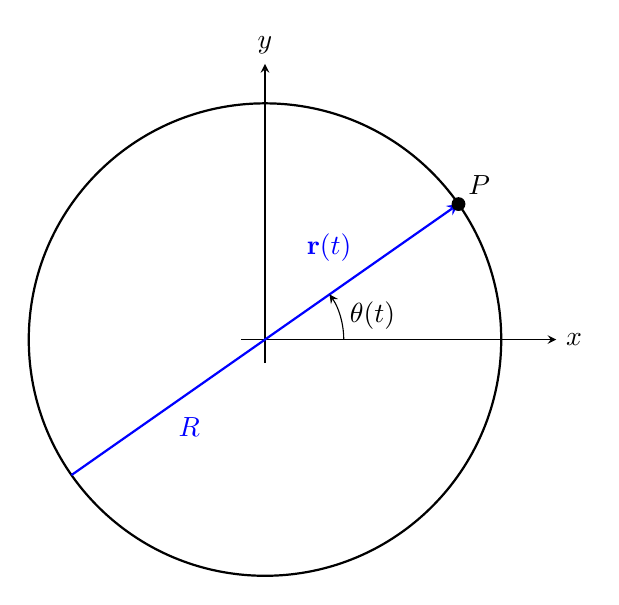
\begin{tikzpicture}[scale=1.0, >=stealth]
        \coordinate (O) at (0,0);
        \coordinate (P) at (35:3);
        \coordinate (PR) at (35:-3);
        \draw[thick] (O) circle (3);
        \draw[->] (-0.3,0) -- (3.7,0) node[right] {$x$};
        \draw[->] (0,-0.3) -- (0,3.5) node[above] {$y$};
        \draw[->,thick,blue] (O) -- (P) node[midway,above left] {$\mathbf{r}(t)$};
        \draw[-,thick,blue] (O) -- (PR) node[midway,below right] {$R$};
        \fill (P) circle (2.5pt) node[above right] {$P$};
        \draw[->] (1,0) arc[start angle=0,end angle=35,radius=1]
            node[midway,right] {$\theta(t)$};

    \end{tikzpicture}
    \caption{Circular path and polar-coordinate vectors at the particle's position.}
\end{figure}
\[
\mathbf{r}(t) = R \cos[\theta(t)] \mathbf{i} + R \sin[\theta(t)] \mathbf{j}
\]
Here, $R$ is the radius of the circular path, and $\theta(t)$ is the angle made by the position vector with respect to a reference axis. We know that $\theta$ changes with time, so it can be represented as a function of time:
\[
\theta = \theta(t)
\]
There is no mathematical restriction on the form of $\theta(t)$, so it can be any function of time. However, if we are interested in \emph{uniform circular motion}, where the speed of the particle is constant, the angle $\theta$ is defined as a linear function of time:
\[
\theta(t) = \omega t + \theta_0
\]

\textbf{What is 1 radian?} A radian is a unit of angular measure used in mathematics and physics. It is defined as the angle subtended at the center of a circle by an arc whose length is equal to the radius of the circle. In other words, if you take a circle and draw an arc that has the same length as the radius of the circle, the angle formed at the center of the circle by that arc is 1 radian.

\begin{figure}[ht]
    \centering
    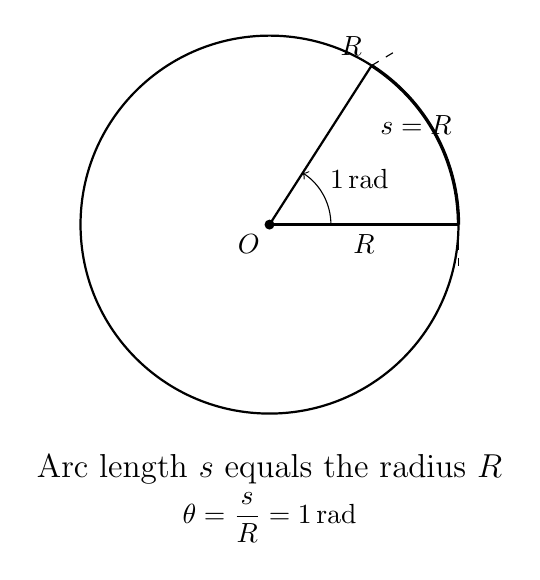
\begin{tikzpicture}[scale=1.2]

        % Circle
        \draw[thick] (0,0) circle (2);

        % Center
        \fill (0,0) circle (1.5pt);
        \node[below left] at (0,0) {$O$};

        % Radius to initial point
        \draw[thick] (0,0) -- (2,0);
        \node[below] at (1,0) {$R$};

        % Radius to final point
        \draw[thick] (0,0) -- ({2*cos(57.3)},{2*sin(57.3)});

        % Arc of length R
        \draw[very thick] (2,0)
            arc[start angle=0, end angle=57.3, radius=2];

        % Angle
        \draw[->] (0.65,0)
            arc[start angle=0, end angle=57.3, radius=0.65];
        \node at (0.95,0.48) {$1\,\mathrm{rad}$};

        % Arc-length label
        \node at (1.55,1.05) {$s=R$};

        % Radius label on second radius
        \node[above left] at ({2*cos(57.3)},{2*sin(57.3)})
            {$R$};

        % Dashed construction showing equal lengths
        \draw[dashed] (2,0) -- (2,-0.45);
        \draw[dashed] ({2*cos(57.3)},{2*sin(57.3)})
            -- ({2*cos(57.3)+0.25},{2*sin(57.3)+0.15});

        % Definition
        \node[align=center] at (0,-2.9)
            {\large Arc length $s$ equals the radius $R$\\[2pt]
             $\displaystyle \theta=\frac{s}{R}=1\,\mathrm{rad}$};

    \end{tikzpicture}
    \caption{Definition of one radian: an angle of $1$ radian subtends an arc whose length equals the radius of the circle.}
    \label{fig:one-radian}
\end{figure}



\subsection{Spiral Motion}

It is a composite motion of linear and circular motions. The particle moves along a spiral path, which can be described by a combination of linear and circular motion equations. The position vector of a particle moving in a spiral path can be expressed as:
\[
\mathbf{r}(t) = r(t) \cos(\theta(t)) \mathbf{i} + r(t) \sin(\theta(t)) \mathbf{j} + z(t) \mathbf{k}
\]


\subsection{Oscillatory Motion}
\emph{Oscillatory motion} is the motion of a particle back and forth around a central point. 

\subsection{Cycloidal Motion}
It is the path traced by a point on the circumference of a circle as it rolls along straight line without slipping. Imagine drawing a chalk dot on a bicycle wheel and then rolling the wheel along a flat surface. The path traced by the chalk dot is a cycloid. 



\section{Worked Examples}
\subsection{Collision of Two Particles}
Two particles are moving on a plane according to the following position vectors:
\[
\mathbf{r}_1(t) = t\mathbf{i} + t\mathbf{j}
\]
\[
\mathbf{r}_2(t) = (-t+4)\mathbf{i} + (2t-2)\mathbf{j}
\]
What time $t$ do the two particles collide? What is the position vector of the collision point?
\textbf{Solution 1:} The two particles collide when their position vectors are equal:
\[
\mathbf{r}_1(t) = \mathbf{r}_2(t)
\]
This gives us two equations:
\[
t = -t + 4 \quad \text{(i)}
\]
\[
t = 2t - 2 \quad \text{(ii)}
\]
From equation (i), we get:
\[
2t = 4 \implies t = 2
\]
From equation (ii), we get:
\[
t = 2t - 2 \implies t = 2
\]
Both equations give us the same time $t = 2$. Now we can find the position vector of the collision point by substituting $t = 2$ into either $\mathbf{r}_1(t)$ or $\mathbf{r}_2(t)$:
\[
\mathbf{r}_1(2) = 2\mathbf{i} + 2\mathbf{j} = 2\mathbf{i} + 2\mathbf{j} 
\]

\textbf{Solution 2:} Define a \emph{seperation vector} $\Delta\mathbf{r}$:
\[
\Delta\mathbf{r} = \mathbf{r}_2(t) - \mathbf{r}_1(t)
\]
The two particles collide when $|\Delta\mathbf{r}| = 0$:
\[
|(-2t+4)\mathbf{i} + (t-2)\mathbf{j}| = 0
\]
This is equivalent to:
\[
\sqrt{(-2t+4)^2 + (t-2)^2} = 0
\]
Squaring both sides:
\[
(-2t+4)^2 + (t-2)^2 = 0
\]
Expanding:
\[
4t^2 - 16t + 16 + t^2 - 4t + 4 = 0
\]
Combining like terms:
\[
5t^2 - 20t + 20 = 0
\]
Dividing by 5:
\[
t^2 - 4t + 4 = 0
\]
This factors as:
\[
(t-2)^2 = 0
\]
So $t = 2$.




\end{document}
